\chapter{Algoritmos Cuánticos}
Las computadoras cuánticas prometen resolver problemas intratables para las computadoras clásicas. Una aplicación es la simulación cuántica. Por ejemplo: simular procesos químicos, que en realidad son procesos cuánticos. Otras posibles aplicaciones incluyen optimización, criptografía y aprendizaje automático. Hay muchos esfuerzos para tratar de aplicar la computación cuántica, pero muchos siguen siendo escépticos. No debemos asumir garantías en las aplicaciones de las computadoras cuánticas, pero seguir explorando las posibilidades.

En este capítulo veremos algunos algoritmos cuánticos famosos que impulsaron el desarrollo de la computación cuántica y que proporcionan una aceleración sobre los algoritmos clásicos, como por ejemplo el algoritmo de Shor para factorizar enteros y el algoritmo de Deutch-Jozsa para determinar si una función booleana está balanceada o no balanceada.

\section{Teleportación Cuántica}

Transferir un estado cuántico de un sistema local (Ej. remoto) a través
del entrelazamiento. Entonces es una nueva forma de comunicación. 

Parte de un circuito como el de la clase pasada haces evolucionar
el estado producto y sale un entrelazado como $\KET{\psi_{AB}}$ entonces
esos dos qubits que en su momento no interactuaron cuánticamente salen
entrelazados pero uno fue a un lugar y el otro a otro (los dos caminos
de abajo). Esto se puede usar para transmitir un estado? Propongo
un 3er estado $\KET{\varphi_{C}}=\alpha\KET 0+\beta\KET 1$.

El sistema parte de un estado (\textbf{etapa }I)
\[
\KET{\psi_{CAB}}=\PARENTESIS{\alpha\KET 0+\beta\KET 1}\PARENTESIS{\underset{AB}{\KET{00}}+\KET{11}}/\sqrt{2}
\]

Hacer alguna operación en el planeta A (involucra 2 canales cuánticos,
los dos de arriba) y que el estado $\KET{\psi_{C}}$ aparezca en el
planeta B. La idea es aplicar una medida de Bell (transforma estados
de Bell en estados productos). El entrelazamiento no es espacial si
están a largas distancias mientras el estado no interactuó con otra
cosa no se pierde.

\begin{quantikz}[slice all] \lstick[wires=2]{$\text{Planeta A}$} & \lstick{$\ket{\varphi_c}=\alpha\ket{0}+\beta\ket{1}$}& \ctrl{1} & \gate{H} & & \ctrl{2}&\qw\\ \qw&\qw&\octrl{-1}&\qw&\ctrl{1}&\qw&\qw\\ \lstick[wires=1]{$\text{Planeta B }\ket{\psi_{AB}}=\frac{\ket{00}+\ket{11}}{\sqrt{2}}$}&\qw&\qw&\qw&\gate{\sigma_x}&\gate{\sigma_x}&\rstick{$\ket{\varphi_c}$} 
\end{quantikz}
\begin{center}
\par\end{center}

\textbf{Etapa intermedia II }

Entre el Control-NOT y el Hadamard

\[
\frac{\alpha}{\sqrt{2}}\KET 0\PARENTESIS{\KET{00}+\KET{11}}+\frac{\beta}{\sqrt{2}}\KET 0\PARENTESIS{\KET{10}+\KET{01}}
\]

\textbf{Etapa III}

Después del Hadamard $H\KET 0=\frac{\KET 0+\KET 1}{\sqrt{2}}$ y $H\KET 1=\frac{\KET 0-\KET 1}{\sqrt{2}}$.
Entonces el estado evoluciona a 

\[
\frac{\alpha}{\sqrt{2}}\frac{\KET 0+\KET 1}{\sqrt{2}}\PARENTESIS{\KET{00}+\KET{11}}+\frac{\beta}{\sqrt{2}}\frac{\KET 0-\KET 1}{\sqrt{2}}\PARENTESIS{\KET{10}+\KET{01}}
\]

(todo esto hecho localmente en A)

Si juntamos todo 

\[
=\frac{1}{2}\CORCHETES{\underset{AC}{\KET{00}}\LLAVEABAJO{\PARENTESIS{\alpha\underset{B}{\KET 0}+\beta\underset{B}{\KET 1}}}{\KET{\varphi}}+\KET{01}\LLAVEABAJO{\PARENTESIS{\alpha\KET 1+\beta\KET 0}}{\sigma_{x}\KET{\varphi}}+\KET{10}\LLAVEABAJO{\PARENTESIS{\alpha\KET 0-\beta\KET 1}}{\sigma_{z}\KET{\varphi}}+\KET{11}\LLAVEABAJO{\PARENTESIS{\alpha\KET 1-\beta\KET 0}}{\sigma_{x}\sigma_{z}\KET{\varphi}}}
\]

Entonces si uno después de esto mide en A $\KET{00}$en B aparece
el $\KET 0$.

Lo que vemos es que como consecuencia el estado c o bien paso al otro
lado tal cual o bien paso al otro lado transformado con algún $\sigma_{\nu}$.
Entonces para hacer que el estado original aparezca en el otro planeta
hay 2 opciones:

- Si están cerca y sólo quiero transferir de un cable al otro es hacer
un control si esta $\KET{00}$ no hago nada o si hay $\KET{01}$ hago
$\sigma_{x}$, así sucesivamente (usando que $\sigma_{\nu}^{2}=I$->
anulo la transformación) y así tendría en B en el estado $\KET{\varphi}$.

Si pongo un Control-X $\sigma_{x}$ y un control z, Si está en 1 le
aplica $\sigma_{x}$ ahora en el otro si esta $\KET 1$ aplica $\sigma_{z}$
ahora bien si está en los dos entonces actual los dos. Entonces con
este esquema en la etapa cuatro obtengo en el último canal $\KET{\varphi_{c}}$.
Puedo decir que el entrelazamiento entre A y B se terminó porque se
usó para transferir el estado $\KET{\varphi_{B}}=\alpha\KET 0+\beta\KET 1$. 

Una forma efectiva es modificar el circuito haciendo una medida $\CheckedBox$,
luego esta $\sigma_{x}^{i}$ siendo $i=0,1$ entonces aplica o no
aplica, esto significa una comunicación clásica (la raya doble),
llamo y le digo tenés que aplicar la medida. Hago lo mismo con $\sigma_{z}$.
 
 $\begin{array}{c} \text{Planeta A} \left\{ \begin{array}{c} \\ \\ \\ \\ \end{array}\right.\\ \text{Planeta B} \end{array}$  \begin{quantikz}[slice all]&\lstick{$\ket{\varphi}_C=\alpha\ket{0}+\beta\ket{1}$}  & \ctrl{1} & \gate{H}&\qw & \meter{}& \cwbend{2}\\  &\lstick{$\ket{\Phi}_A^+$}&\targ{}&\qw&\meter{} &\cwbend{1}\\  &\lstick{$\ket{\Phi}_B^+$}&\qw& \qw &\qw&\targ{}& \ctrl{} \end{quantikz}

Se usa cristal birrefringente uno de los fotones queda en la tierra
el otro se manda al satélite se hacen las cosas y se prueba esto.

Esto muestra que el entrelazamiento nos permite una nueva forma de
comunicación.

Si hago traza parcial en el canal B antes de los sigmas, 
\[
\rho_{B}=Tr_{AC}\PROYECT{\psi_{CAB}}{\psi_{CAB}}=\frac{\PROYECT 00+\PROYECT 11}{0}
\]

Luego voy a obtener el estado puro $\KET{\varphi}$.

Si hubiera un estado D entrelazado con C, luego de aplicar todo esto
terminaría teniendo el estado D entrelazado con B.

\section{Codificación Superdensa}

La codificación superdensa permite ver de manera simple que si dos partes, Alice y Bob,
comparten un estado entrelazado de la forma: 

% Dada una fuente que emite un par de fotones o qubits entrelazados
\[
\KET{\psi_{AB}}=\frac{\KET{00}+\KET{11}}{\sqrt{2}}
\]

Alice puede enviar dos bits de información, operando solmente sobre su qubit y enviándolo,
nuevamente para hacer una medida. 

Esquematicamente podemos considerar que una fuente que emite un par de fotones,
en A hacemos una operación U sobre ese qubit. Luego A envía su qubit para hacer
una medida conjunta en estos dos cables cuánticos.

\begin{center}
\includegraphics[scale=0.5]{\string"fig3 clase4-9\string".png}
\par\end{center}

Si A desea enviar $'00'$,  aplica la I, entonces el estado queda igual $\KET{\psi_{AB}}=\frac{\KET{00}+\KET{11}}{\sqrt{2}}$. 

Si A desea enviar $'01'$, aplica $\sigma_{z}$, entonces $\KET{\psi_{AB}}\rightarrow\frac{\KET{00}-\KET{11}}{\sqrt{2}}$

Si A desea enviar $'10'$, aplica $\sigma_{x}$, entonces $\KET{\psi_{AB}}\rightarrow\frac{\KET{10}+\KET{01}}{\sqrt{2}}$

Si A desea enviar $'11'$, aplica $i \sigma_{y}=\sigma_{z} \sigma_{x}$, $\KET{\psi_{AB}}\rightarrow\frac{\KET{10}-\KET{01}}{\sqrt{2}}$

De esta forma se obtienen los $4$ estados ortogonales de la base de Bell 
por lo que son distinguibles.

% Luego se realiza la medida conjunta y se observan que llego a 4 estados ortogonales
% bien distinguidos, entonces si puedo medir estados Bell, pero si recibo
% el qubit que viene de A como esta entrelazado voy a poder ver la operación
% que hice y voy a obtener 2 bits de información 1 de la operación que
% hice y 1 del estado.

% Entonces vemos que el entrelazamiento lo podemos usar para transmitir
% información. 

% Para medir en base estándar mido la polarización directo o con un
% stern y gerlach. Ahora bien si quiero hacer medida en la base de Bell,
% lo que hago antes de medirlo 

Si se quiere realizar la medida en la base computacional, se le aplica la 
siguiente operación para pasarlo de la base de Bell a la computacional: primero
control not y después la Hadamard 

\begin{quantikz}  && \text{Medida de Bell} &&\\ \qw  & \ctrl{1} & \gate{H}&\qw & \meter{}\\   \qw&\targ{}&\qw&\qw &\meter{} \end{quantikz}

Notando que $(AB)^{-1}=B^{-1}A^{-1}$ y dado
que las inversas de la Control-NOT y de la compuerta Hadamard
son la misma compuerta, se puede invertir como indica la figura. 

\section{El primer algoritmo (histórico) Deutsch 1986.}

La idea es tomar el problema más simple posible donde la mecánica cuántica pueda hacer algo que lo clásico no. Dada una función $f:\LLAVES{0,1}\rightarrow\LLAVES{0,1}$, la pregunta que me hago: $f(0)=f(1)$ o $f(0)\neq f(1)$. Clásicamente necesita dos evaluaciones de la función pero cuánticamente lo podemos
hacer en una sola evaluación.

Planteo un sistema de dos qubits pero pongo un bloque grande que implica una operación no sobre un sólo qubit sino una operación que involucra ambos qubits. Es decir hacerlo con una sóla entrada

Sabemos que $f(0)=0\:o\:1$ al igual que $f(1)$. $U_{f}\KET{ij}=\KET{i,j\oplus f(i)}$
con $\oplus$ suma en módulo 2. Podemos ver que $U_{f}$ es unitaria. 
\begin{center}
\begin{quantikz}  &\rstick{$\frac{\ket{0}+\ket{1}}{\sqrt{2}}$} &\\ \lstick{$\ket{0}$}&\gate{H}&\qw& \gate[wires=2]{U} &\qw \\ \lstick{$\ket{1}$}&\gate{H}&\qw& &\qw \\ & \rstick{$\frac{\ket{0}-\ket{1}}{\sqrt{2}}$} &\\ \end{quantikz}  $\frac{\ket{0}+\ket{1}}{\sqrt{2}}\frac{\ket{0}}{\sqrt{2}}(-1)^{f(0)}+\frac{\ket{0}-\ket{1}}{\sqrt{2}}\frac{\ket{1}}{\sqrt{2}}(-1)^{f(1)}$ 
\par
\end{center}

Entonces qué pasa 
\[
\KET 0\PARENTESIS{\frac{\KET 0-\KET 1}{\sqrt{2}}}=\frac{\KET{00}-\KET{01}}{\sqrt{2}}\underset{U_{f}}{\rightarrow}\frac{U_{f}\KET{00}-U_{f}\KET{01}}{\sqrt{2}}
\]

\[
=\KET{0,f(0)}-\KET{0,1\oplus f(0)}=\KET 0\PARENTESIS{\KET{f(0)}-\KET{1\oplus f(0)}}=(-1)^{f(0)}\KET 0\frac{\KET 0-\KET 1}{\sqrt{2}}
\]

Si $f(0)$ es 0 queda el estado original

Si $f(0)=1$ queda menos el estado original

Ahora bien el resultado de esta suma es

\[
\frac{1}{2}\PARENTESIS{\KET 0(-1)^{f(0)}+\KET 1(-1)^{f(1)}}\PARENTESIS{\KET 0-\KET 1}
\]
es decir uno obtiene el valor de $f$ como una fase. 

\[
\frac{1}{2}(-1)^{f(0)}\PARENTESIS{\KET 0+\KET 1(-1)^{f(1)-f(0)}}\PARENTESIS{\KET 0-\KET 1}
\]
Ahí vimos que se puede hacer en un sólo paso. La fase que tenemos
sobre todo el estado no nos importa, ahora bien si $f(0)=f(1)$ entonces
me devuelve el estado original, ahora si $f(0)\neq f(1)$ me da el
estado ortogonal. Mido en la base de x entonces si me da 1 son iguales
si me da -1 son distintas. Vuelvo a ponerlo en la base computacional
con una Hadamard, y obtengo

\begin{center}
 \begin{quantikz}  &\rstick{$\frac{\ket{0}+\ket{1}}{\sqrt{2}}$} &\\ \lstick{$\ket{0}$}&\gate{H}&\qw& \gate[wires=2]{U} &\qw\rstick{$\ket{0}\quad f(0)=f(1)$\\$\ket{1}\quad f(0)\neq f(1)$} \\ \lstick{$\ket{1}$}&\gate{H}&\qw& &\qw \\ & \rstick{$\frac{\ket{0}-\ket{1}}{\sqrt{2}}$} &\\ \end{quantikz}     
\end{center}


¿Quién es $U_{f}$?

Si $f(0)=f(1)=0$ es la I  \begin{quantikz}  \qw&\qw\\ \qw&\qw \end{quantikz}   

Si $f(0)=f(1)=1$ es $I_{A}\otimes\sigma_{xB}$ \begin{quantikz} \rstick{$I_A\otimes\sigma_{xB}$}\\ \qw&\qw&\qw\\ \qw&\gate{X}&\qw\end{quantikz}   

Si $f(0)=0$, $f(1)=1$ control not \begin{quantikz}  \qw&\ctrl{1}&\qw\\ \qw&\targ{}&\qw\end{quantikz}  
$\PROYECT 00\otimes I_{B}+\PROYECT 11\otimes\sigma_{x}$

Si $f(0)=1$, $f(1)=0$ un control not dado vuelta (el circulo chiquito
implica 2 $\sigma_{x}$) 

\begin{quantikz}  \qw&\octrl{1} &\qw\\ \qw&\targ{}&\qw\end{quantikz} = \begin{quantikz}  \gate{X}&\ctrl{1} &\gate{X} \qw\\ \qw&\targ{}&\qw\end{quantikz} 

\section{Algoritmo de Deutsch - Jozsa}

Ahora tengo $f:\{0,1\}^{\otimes n}\rightarrow\LLAVES{0,1}$ ie $f:\LLAVES{0,1,\dots,2^{n}-1}\rightarrow\LLAVES{0,1}$

$f$ puede ser constante $f(i)=0$ $\forall i$ o $f(i)=1$ $\forall i$
o balanceada $f(i)=0$ para mitad del dominio y $f(i)=1$ la otra
mitad. 

\textbf{Clásicamente:} para saber si $f$ es constante o balanceada se necesitan 
$\frac{2^{n}}{2}+1$ evaluaciones de $f$. Es exponencialmente grande.

\textbf{Cuánticamente:} se necesita una evaluación de $f$. 

¿ Cómo es el circuito?
\begin{center}
\begin{quantikz} \lstick[wires=4]{N-1} & \lstick{$\ket{0}$} & \gate{H} &  \gate[5]{U_f} & \gate{H} &\meter{} \\ & \lstick{$\ket{0}$} & \gate{H} &   & \gate{H} &\meter{} \\ & \lstick{$\ket{0}$} & \gate{H} &   & \gate{H} &\meter{} \\ & \lstick{$\ket{0}$} & \gate{H} &   & \gate{H} &\meter{} \\ \qw&\lstick{$\ket{1}$} & \gate{H} &   & \gate{H} &\meter{} \\ \end{quantikz}
\par
\end{center}

$H^{\otimes n}\KET{00\dots0}=H\KET 0H\KET 0\otimes H\KET 0=\PARENTESIS{\KET 0+\KET 1}\PARENTESIS{\KET 0+\KET 1}\otimes\dots\PARENTESIS{\KET 0+\KET 1}$

\[
=\KET{0\dots0}+\KET{0\dots01}+\dots=\sum_{j=0}^{2^{n}-1}\KET j
\]

esta es la base binaria

$U_{f}\KET{j,i}=\KET{j,i\oplus f(j)}$ luego si aplico $U_{f}\KET -=\KET -\:o\:-\KET -$. 

El estado 
\[
\underset{\KET{0\dots0}}{\KET 0}\KET 1\rightarrow\sum_{j=0}^{2^{n}-1}\KET j\KET -\underset{U_{f}}{\rightarrow}\sum_{j=0}^{2^{n}-1}\KET j(-1)^{f(j)}\KET -
\]

Habíamos dicho que $f(j)$ podía ser constante o balanceada, entonces cómo
nos damos cuenta en que caso estamos:


Constante: $\PARENTESIS{\sum_{j=0}^{2^{n}-1}\KET j}\KET -(-1)^{f(1)}\rightarrow\KET 0\KET -(-1)^{f(1)}$
Balanceada: $\KET 1\KET -$

En resumen este circuito con una sola entrada genera todos estados
ortogonales, si $f$ es constante mido y me van a dar todos los qubits para
arriba ahora si $f$ es balanceada alguno me va a dar hacia abajo.

\textbf{¿Cuántos gates necesito para hacerlo? }vamos a ver que no
necesito tantos.

\section{Algoritmos para estados mezcla - Knill Laflamme 1998 (Deterministic
quantum computation with one qubit - DQCL)}


Tenemos el circuito,
\begin{center}
\begin{quantikz}  \lstick{$\ket{0}$} & \gate{H} & \qw & \ctrl{1} & \qw   & \rstick{$\begin{matrix} \langle \sigma_x \rangle=Re(Tr U)\\ \langle \sigma_y \rangle=Im(Tr U) \end{matrix}$} \qw  \\ \lstick{$\frac{I_{2^n}}{(\sqrt{2})^n}$} &\qwbundle[alternate]{}&\qwbundle[alternate]{}&\gate{U}\qwbundle[alternate]{} & \qwbundle[alternate]{}  \end{quantikz} 
\end{center}

entra un estado $\frac{I_{2^{n}}}{(\sqrt{2})^{n}}$
cualquiera que puede ser mezcla. A la salida mido $\VALMEDIO{\sigma_{x}}$,
$\VALMEDIO{\sigma_{y}}$ esto te da la $Re\PARENTESIS{TrU}$ y la
$Im\PARENTESIS{TrU}$, respectivamente. Esto nos permitiría evaluar
directamente la $TrU$ sin mucha dificultad, lo cual para un sistema
de $n$ qubits es difícil. 

\[
\rho_{AB}\begin{cases}
\begin{array}{c}
\rho_{sep}\begin{cases}
\begin{array}{c}
\text{producto }\rho_{A}\otimes\rho_{B}\\
\text{clásicamente correlacionados }\rho_{AB}=\sum_{ij}p_{ij}\PROYECT{ij}{ij}\\
\rho_{AB}=\sum_{\alpha}p_{\alpha}\rho_{A}^{\alpha}\otimes\rho_{B}^{\alpha}
\end{array} & \begin{array}{c}
\\
\text{1eros 2: clásicos}\\
\text{caso intermedio}
\end{array}\end{cases}\\
\begin{array}{cc}
\text{no separables o entrelazados} & \text{caso cuántico}\end{array}
\end{array}\end{cases}
\]
Las razones por las cuales por las que los estados mezclas se volvieron
importantes es por su aplicación en los algoritmos de Mill y Billamar,
porque se puede hacer computación cuántica con estados mezcla, con
mucho ruido y a temperatura ambiente. 

\begin{quantikz}  \lstick{$\ket{0}$} & \gate{H} & \qw &  \ctrl{1} & \qw   &\meter {}  \\ &\lstick{$\frac{I_{2^n}}{(\sqrt{2})^n}$} &\qwbundle[alternate]{}&\gate{U}\qwbundle[alternate]{} & \qwbundle[alternate]{}  \end{quantikz} 

En el canal 1 luego de la Hadamard tenemos el estado $\KET +=\frac{\KET 0+\KET 1}{\sqrt{2}}$
y en los otros antes de la compuerta U tenemos el estado $\KET{\psi}$

$\PARENTESIS{\frac{\KET 0+\KET 1}{\sqrt{2}}}\otimes\KET{\psi}\rightarrow\LLAVEABAJO{\PARENTESIS{\KET 0\KET{\psi}+\KET 1U\KET{\psi}}}{\KET{\psi_{AB}}}\frac{1}{\sqrt{2}}$

Luego 
\[
\rho_{A}=Tr_{B}\PROYECT{\psi_{AB}}{\psi_{AB}}Tr_{B}\frac{1}{2}\PARENTESIS{\PROYECT 00\otimes\PROYECT{\psi}{\psi}+\PROYECT 11\otimes U\PROYECT{\psi}{\psi}U^{\dagger}+\PROYECT 01\otimes\PROYECT{\psi}{\psi}U^{\dagger}+\PROYECT 10\otimes U\PROYECT{\psi}{\psi}}
\]

\[
=\frac{1}{2}\PARENTESIS{\PROYECT 00+\PROYECT 11+\PROYECT 01\LLAVEARRIBA{\EXPECT{\psi}{\psi}{U^{\dagger}}}{\psi\text{ es base de }U}+\PROYECT 10\EXPECT{\psi}{\psi}U}
\]

Si ahora hago 
\[
\VALMEDIO{\sigma_{x}^{A}}=Tr\PARENTESIS{\rho_{A}\sigma_{x}}=\EXPECT{\psi}{\psi}{U^{\dagger}}+\EXPECT{\psi}{\psi}U=2Re\EXPECT{\psi}{\psi}U
\]

\[
\VALMEDIO{\sigma_{y}^{A}}=Tr\PARENTESIS{\rho_{A}\sigma_{y}}=\EXPECT{\psi}{\psi}U/i-\EXPECT{\psi}{\psi}{U^{\dagger}}/i=2Im\EXPECT{\psi}{\psi}U
\]

Ahora cuando aplico esto a una mezcla estadística de estados, a la
salida tengo una mezcla estadística de estados.

La idea ahora es poner un $\rho=\sum_{i}p_{i}\PROYECT{\psi_{i}}{\psi_{i}}$,
lo que vamos a obtener de todo esto, como es lineal, el resultado
va a ser la mezcla estadística de todo.

\[
\rho_{iA}=\frac{1}{2}\PARENTESIS{\PROYECT 00+\PROYECT 11+\PROYECT 01\EXPECT{\psi}{\psi}{U^{\dagger}}+\PROYECT 10\EXPECT{\psi}{\psi}U}
\]

\[
\rho_{A}=\sum_{i}p_{i}\rho_{iA}=\frac{1}{2}\PARENTESIS{\PROYECT 00+\PROYECT 11+\PROYECT 01\sum_{i}p_{i}\VALMEDIO{U^{\dagger}}_{i}+\PROYECT 10\sum_{i}p_{i}\VALMEDIO U_{i}}
\]

Si ahora $\rho_{B}^{0}=\frac{1}{2^{n}}\sum_{i}\PROYECT{\psi_{i}}{\psi_{i}}=\frac{1}{2^{n}}I_{B}$,
es decis mandamos un estado completamente mezclado, temperatura infinita
(cra la dif de energía entre niveles, temp ambiente)

Entonces, ahora como los $p_{i}$ son todos iguales 
\[
\rho_{A}=\frac{1}{2}\PARENTESIS{\PROYECT 00+\PROYECT 11+\PROYECT 01\sum_{i=1}^{2^{n}}\frac{\EXPECT ii{U^{\dagger}}}{2^{n}}+\PROYECT 10\sum_{i=1}^{2^{n}}\frac{\EXPECT iiU}{2^{n}}}
\]

\[
\rho_{A}=\frac{1}{2}\PARENTESIS{\PROYECT 00+\PROYECT 11+\PROYECT 01\PARENTESIS{\frac{TrU}{2^{n}}}^{*}+\PROYECT 10\PARENTESIS{\frac{TrU}{2^{n}}}}
\]

Ahora estoy facilitándome la cuenta de la $TrU$, cuando $U$ es muy
grande. Solo necesito hacer muchas veces (ej 100) el circuito para
obtener el $\VALMEDIO{\sigma_{x}}$, $\VALMEDIO{\sigma_{y}}$. Volvemos
a obtener que 

\[
\VALMEDIO{\sigma_{x}}=Tr\PARENTESIS{\rho_{A}\sigma_{x}}=2ReTr\PARENTESIS U/2^{n}
\]

\[
\VALMEDIO{\sigma_{y}}=Tr\PARENTESIS{\rho_{A}\sigma_{y}}=2ImTr\PARENTESIS U/2^{n}
\]

Entonces cuando meto 
\[
\frac{I_{B}}{2^{n}}\rightarrow U\frac{I_{B}}{2^{n}}U^{\dagger}=\frac{I_{B}}{2^{n}}\qquad UU^{\dagger}=I_{B}
\]
uno medio naive piensa que no sirve para nada, pero en realidad la
importancia está en los términos cruzados. 

En esto tenemos entrelazamiento, o tenemos muy poco, entonces este
estado es tipo separable y pensaban que esto es simulable clásicamente,
pero no es así, por lo que esta diciendo que los estados mezcla tiene
algunas propiedades que no tienen los estados clásicos. El recurso
que está atrás se llama \emph{discord} que no está terminado de estudiar. 

Este algoritmo inauguró lo que se llama mixed state q.c, lo tradicional
es pure state q.c.

\subsection{¿Qué pasa si el qubit de control en vez de ser puro es mezcla?}

Veamos primero que sucede si pongo a la entrada un $\KET 1\overset{H}{\rightarrow}\frac{\KET 0-\KET 1}{\sqrt{2}}$,
lo que va a quedar si hacemos toda la cuenta es que el

\[
\rho_{A}=\frac{1}{2}\PARENTESIS{\PROYECT 00+\PROYECT 11-\PROYECT 01\PARENTESIS{\frac{TrU}{2^{n}}}^{*}-\PROYECT 10\PARENTESIS{\frac{TrU}{2^{n}}}}
\]

\[
\VALMEDIO{\sigma_{x}}=Tr\PARENTESIS{\rho_{A}\sigma_{x}}=-Re\EXPECT{\psi}{\psi}U
\]

Ahora sup que entramos con una mezcla $p\PROYECT 00+q\PROYECT 11$,
con $q=1-p$
\begin{center}
\begin{quantikz}  &\rstick{$\downarrow \ket{+}=\frac{\ket{0}\pm\ket{1}}{\sqrt{2}}$}\\ \lstick{$p\ket{0}\bra{0}+q\ket{1}\bra{1} $}&\gate{H}&\ctrl{1}&\meter{}&\qw\rstick{$\langle\sigma_x\rangle=Re\left(\frac{Tr(U)}{2^n}\right)$\\$\langle\sigma_y\rangle=IM\left(\frac{Tr(U)}{2^n}\right)$}\\ &\lstick[wires=3]{$\frac{I_B}{2^n}$}& \gate{U_x}\qwbundle[alternate]{} & \qwbundle[alternate]{} \end{quantikz} 
\par
\end{center}

\[
\rho_{A}=\frac{1}{2}\PARENTESIS{\PROYECT 00+\PROYECT 11+\PARENTESIS{p-q}\PROYECT 10\EXPECT{\psi}{\psi}U+\PARENTESIS{p-q}\PROYECT 01\EXPECT{\psi}{\psi}{U^{\dagger}}}
\]

Lo que aparece es un valor medio cada vez más débil cuando $p\rightarrow q$. 

\[
\VALMEDIO{\sigma_{x}}=Re\CORCHETES{\EXPECT{\psi}{\psi}U}\PARENTESIS{p-q}
\]
\[
\VALMEDIO{\sigma_{y}}=Im\CORCHETES{\EXPECT{\psi}{\psi}{U^{\dagger}}}\PARENTESIS{p-q}
\]

Ahora si metemos uno completamente mezclado 
\[
\VALMEDIO{\sigma_{x}}=\PARENTESIS{p-q}Re\PARENTESIS{\frac{TrU}{2^{n}}}
\]
\[
\VALMEDIO{\sigma_{y}}=\PARENTESIS{p-q}Im\PARENTESIS{\frac{TrU}{2^{n}}}
\]

Entonces puedo hacer algunos algoritmos de forma eficiente con estados
mezclas. 

Esta es otra forma de escribir esto:

\begin{center}
    \begin{quantikz}  
\lstick{$\rho
_A$} & \gate{H} & \qw & \ctrl{1} & \qw   &\meter {} & \rstick{$\begin{matrix} \langle \sigma_x \rangle=(p-q)Re(\frac{Tr U}{2^n})\\ \langle \sigma_y \rangle=(p-q)Im(\frac{Tr U}{2^n}) \end{matrix}$} \qw  \\
\lstick{$\rho_B$} &\qwbundle[alternate]{}&\qwbundle[alternate]{}&\gate{U}\qwbundle[alternate]{} & \qwbundle[alternate]{}  
\end{quantikz} 
\end{center}

Es fácil de implementar con fotones. 

\section{Transformada de Fourier Cuántica}
Una operación muy importante, tanto en computación clásica como cuántica es la \emph{Transformada de Fourier}. La transformada de Fourier transforma de una función $f(t)$ en el dominio temporal a otra función  $F(x)$ en el dominio de frecuencia. Naturalmente la transformación inversa se obtiene a partir de la transformada de Fourier \emph{inversa}. Si observamos, a modo de ejemplo, el gráfico de la función $\cos(t)$ que se puede ver en la Figura~\ref{fig:cos_time_graph}, 
donde el eje $x$ se gráfica el tiempo y en el eje $y$ la amplitud. Si se aplica la transformada de Fourier a esta función se obtiene una función en el dominio de frecuencia, como se puede observar en la Figura~\ref{fig:cos_freq_graph}.
\begin{figure}[ht]
  \centering
  \begin{multicols}{2}
    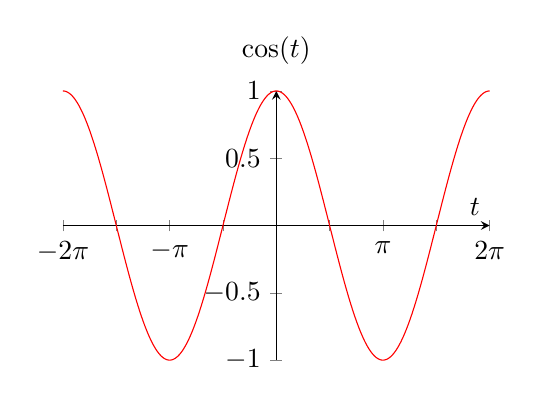
\begin{tikzpicture}
      \begin{axis}[
        title={$\cos(t)$},
        xlabel={$t$},
        axis lines = middle,
        xmax=2*pi,
        xmin=-2*pi,
        height=5cm,
        width=7cm,
        ymin=-1,
        ymax=1,
        xticklabels={$-2\pi$, , $-\pi$, ,
            , $\pi$, , $2\pi$},
        xtick={-6.28318, -4.7123889, -3.14159, -1.5708, 1.5708, 3.14159, 4.7123889, 6.28318}
      ]
        \addplot[red, domain=-2*pi:2*pi, samples=1000]{ cos(deg(x)) };
      \end{axis}
    \end{tikzpicture}
    \caption{Gráfico de $\cos(t)$ en el dominio de tiempo.}
    \label{fig:cos_time_graph}

    \begin{tikzpicture}
      \begin{axis}[
        title={$F(\cos(t))$},
        xlabel={$x$},
        axis lines=middle,
        height=5cm,
        width=6cm,
        xmax=2,
        xmin=-2,
        ymin=0,
        ymax=2
      ]
         \addplot[ycomb, blue, mark=, thick, mark=*] coordinates {
          (1, 1) (-1, 1)
         };
      \end{axis}
    \end{tikzpicture}
    \caption{Gráfico de $F(\cos(t))$ en el dominio de frecuencia.}
    \label{fig:cos_freq_graph}
  \end{multicols}
\end{figure}

La transformada de Fourier es sumamente útil en el procesamiento de señales. La señal que se muestra en la Figura~\ref{fig:cos_time_graph} es una señal continua por lo que se asume que se extiende hasta el infinito. Sin embargo, las computadoras solo puede trabajar con señales finitas y discretas. Esto implica que se tenga que discretizar las funciones continuas como se ve en la Figura~\ref{fig:cos_discrete_time_graph}. Podemos transformar la señal discreta usando la \emph{transformada de Fourier discreta}.
\begin{figure}[ht]
  \centering
  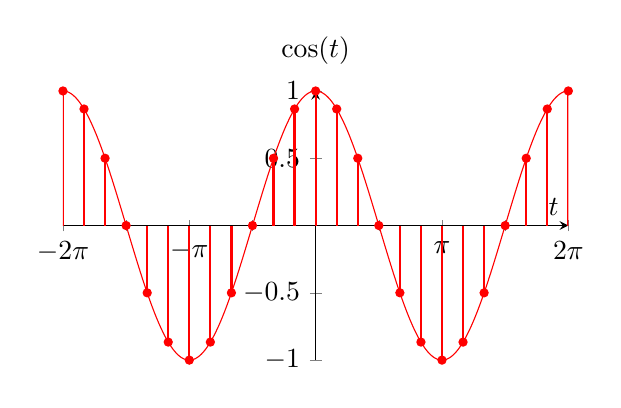
\begin{tikzpicture}
    \begin{axis}[
      title={$\cos(t)$},
      xlabel={$t$},
      axis lines = middle,
      xmax=2*pi,
      xmin=-2*pi,
      height=5cm,
      width=8cm,
      ymin=-1,
      ymax=1,
      xticklabels={$-2\pi$, , $-\pi$, , , $\pi$, , $2\pi$},
      xtick={-6.28318, -4.7123889, -3.14159, -1.5708, 1.5708, 3.14159, 4.7123889, 6.28318}
    ]
      \addplot[ycomb, red, domain=-2*pi:2*pi, samples=25, mark=*, thick, mark size=1.25pt]{ cos(deg(x)) };
      \addplot[red, domain=-2*pi:2*pi, samples=1000, draw]{ cos(deg(x)) };
    \end{axis}
  \end{tikzpicture}
  \caption{Versión discretizada de la función continua $\cos(t)$. Cada punto representa una muestra de la señal. El tiempo entre muestras se denomina tiempo de muestreo.}
  \label{fig:cos_discrete_time_graph}
\end{figure}

La transformada de Fourier discreta se puede ver como una operación lineal. Esto es porque transforma de un vector $N$-dimensional a otro vector $N$-dimensional a través de una matriz de $N \times N$: $F_N$. Para un estado de $n$ qubits, $N$ es igual a $2^n$. Esta transformación se puede escribir como
\begin{equation}
  \ket{x} = \sum_{j=0}^{N-1}x_j\ket{j} \longrightarrow \sum_{k=0}^{N-1}y_k\ket{k},
\end{equation}
donde las amplitudes $y_k$ son las transformadas de Fourier discretas de las amplitudes $x_j$. 
En otras palabras, la transformada de Fourier cuántica (\emph{Quantum Fourier Transform (QFT)}) transforma a los estados de la base estándar de la siguiente manera
\begin{equation} \label{eq:qft}
  F_N\ket{j} = \dfrac{1}{\sqrt N}\sum_{k=0}^{N-1}e^{2\pi i jk/N}\ket{k}.
\end{equation}
Nota que es equivalente a una transformada de Fourier discreta clásica \emph{inversa}. 
La QFT proporciona una aceleración exponencial respecto del algoritmo clásico \emph{FFT:Fast Fourier Transform}.

Ya hemos visto la QFT de un qubit, se trata simplemente de la compuerta Hadamard:
\begin{equation}
  F_2 = H = \hgate.
\end{equation}
Para describir la QFT de $n$-qubits necesitamos las compuertas Hadamard y control fase.
Escribiremos a la compuerta fase como $R_k$ donde
\begin{equation}
  R_k = \begin{pmatrix}
    1 & 0 \\
    0 & e^{2\pi i/2^k}
  \end{pmatrix}.
\end{equation}
En la Figura~\ref{fig: quantum_3_qubit_fourier_circ} se puede observar el circuito para una QFT de 3 qubits. Tener en cuenta que $ S = R_2 $ y $ T = R_3 $. La compuerta cruzada al final es una compuerta de swap, que intercambia dos qubits. El orden de los qubits debe invertirse al final de una QFT para obtener el orden correcto como resultado. De todas formas, invirtiendo el orden de las compuertas y tomando la inversa $ U ^ \ dagger $ de cada compuerta $ U $ da un circuito igualmente eficiente para la transformada cuántica de Fourier inversa $ F_N ^ \ dagger $.

\begin{figure}[ht]
\begin{center}
\begin{quantikz}
\lstick{$\ket{x_0}$} & \gate{H} & \gate{S} & \gate{T} & \qw & \qw & \qw & \swap{2} & \qw \\
\lstick{$\ket{x_1}$} & \qw & \ctrl{-1} & \qw & \gate{H} & \gate{S} & \qw & \qw & \qw \\
\lstick{$\ket{x_2}$} & \qw & \qw & \ctrl{-2} & \qw & \ctrl{-1} & \gate{H} & \targX{} & \qw \\
\end{quantikz}
\end{center}
  \caption{Circuito que realiza la transformada de Fourier cuántica de 3 qubits.}
  \label{fig:quantum_3_qubit_fourier_circ}
\end{figure}
\noindent
Se puede escribir la matriz que implementa la QFT, tomando $\omega = e^{2\pi i/N}$. Para 3 qubits, donde $N = 8$:
\begin{equation}
  F_8 = \dfrac{1}{\sqrt 8}
  \begin{pmatrix}
    1 & 1 & 1 & 1 & 1 & 1 & 1 & 1 \\
    1 & \omega^1 & \omega^2 & \omega^3 & \omega^4 & \omega^5 & \omega^6 & \omega^7 \\
    1 & \omega^2 & \omega^4 & \omega^6 & 1 & \omega^2 & \omega^4 & \omega^6 \\
    1 & \omega^3 & \omega^6 & \omega^1 & \omega^4 & \omega^7 & \omega^2 & \omega^5 \\
    1 & \omega^4 & 1 & \omega^4 & 1 & \omega^4 & 1 & \omega^4 \\
    1 & \omega^5 & \omega^2 & \omega^7 & \omega^4 & \omega^1 & \omega^6 & \omega^3 \\
    1 & \omega^6 & \omega^4 & \omega^2 & 1 & \omega^6 & \omega^4 & \omega^2 \\
    1 & \omega^7 & \omega^6 & \omega^5 & \omega^4 & \omega^3 & \omega^2 & \omega^1 \\
  \end{pmatrix}.
\end{equation}
Un circuito más general para una QFT sobre un estado de $n$ qubits se describe en la Figura~\ref{fig:quantum_fourier_circ}.

\begin{figure}[ht]
\begin{Code}
\begin{center}
\begin{quantikz}[row sep=0.3cm,column sep=0.15cm]%
\lstick{$\ket{x_0}$} & \gate{H} & \gate{R_2} & \qw & \dots & & \gate{R_{n-1}} & \gate{R_n} & \qw & \qw & \qw & \qw & \qw & \qw & \qw & \qw & \qw & \qw & \qw & \qw & \qw \\
\lstick{$\ket{x_1}$} & \qw & \ctrl{-1} & \qw & \dots & & \qw & \qw & \gate{H} & \qw & \dots & & \gate{R_{n-2}} & \gate{R_{n-1}} & \qw & \dots & & \qw & \qw & \qw & \qw \\
\rstick{\vdots} & & & & \vdots & & & & & & & & & & & \\
\lstick{$\ket{x_{n - 1}}$} & \qw & \qw & \qw & \qw & \qw & \ctrl{-3} & \qw & \qw & \qw & \qw & \qw & \ctrl{-2} & \qw & \qw & \dots & & \gate{H} & \gate{R_2} & \qw & \qw \\
\lstick{$\ket{x_n}$} & \qw  & \qw & \qw & \qw & \qw & \qw & \ctrl{-4} & \qw & \qw & \qw & \qw & \qw & \ctrl{-3} & \qw & \dots & & \qw & \ctrl{-1} & \gate{H} & \qw \\
\end{quantikz}
\end{center}
\end{Code}
  \caption{Transformada de Fourier Cuántica sobre $n$ qubits.}
  \label{fig:quantum_fourier_circ}
\end{figure}

El resultado de la transformada de Fourier del estado original se almacena en la amplitudes. 
Sin embargo, recordar que estas amplitudes no se pueden extraer. Por tanto, no hay forma de determinar la transformada de Fourier del estado original usando QFT\@. Aunque no podemos extraer los valores transformados después de una QFT, la QFT tiene su uso en algoritmos cuánticos como el algoritmo de Shor para factorizar enteros y el algoritmo de estimación de fase cuántica.
\newpage

\section{Algoritmo Cuántico de Estimación de Fase}
El algoritmo cuántico de estimación de fase (\emph{QPE} por sus siglas en inglés: Quantum Phase Estimation), estima la fase de un autovector de un operador unitario. Si se prepara un autoestado  $\ket{u}$ de un operador unitario $U$, donde $U\!\ket{u} = e^{2\pi i \varphi}\ket{u}$ 
y el valor de $\varphi$ es desconocido ($0 \le \varphi \le 1$). 
El objetivo es determinar el valor de $\varphi$ 
donde no se conoce necesariamente ni $U$ ni $\ket{u}$, 
pero se tienen cajas negras capaces de preparar $\ket{u}$ 
y aplicar operaciones control-$U$.


\begin{figure}[ht]
\begin{Code}
\begin{center}
\begin{quantikz}[row sep=0.3cm,column sep=0.65cm]%
\lstick{$\ket{0}$} & \gate{H} & \qw & \qw & \qw & \dots & & \ctrl{4} & \gate[4, nwires={2}]{\,F^\dagger_n\,} & \qw & \meter{} & \cw \\
\rstick{\vdots} & & & \vdots & & & & & & & \vdots \\
\lstick{$\ket{0}$} & \gate{H} & \qw & \ctrl{2} & \qw & \dots & & \qw & & \qw & \meter{} & \cw \\
\lstick{$\ket{0}$} & \gate{H} & \ctrl{1} &  \qw & \qw & \dots & & \qw & & \qw & \meter{} & \cw \\
\lstick{$\ket{u}$} & \qw\qwbundle{m} & \gate{U^{2^0}} & \gate{U^{2^1}} & \qw & \dots & & \gate{U^{2^{n-1}}} & \qw & \qw & \qw & \qw \\
\end{quantikz}
\end{center}
\end{Code}
\caption{Circuito del algoritmo de estimación de fase, donde $F^\dagger_n$ 
representa la inversa de la transformada de Fourier de $n$ qubits. La ``/" denota $m$ qubits.}
  \label{fig:phase_estimation_circ}
\end{figure}

El circuito del algoritmo QPE que se observa en la Figura~\ref{fig:phase_estimation_circ} consiste de dos registros. Los $n$ qubits superiores comprenden el primer registro que se utilizará para calcular la estimación de $\varphi$. El tamaño del primer registro se puede elegir en función de dos factores: precisión y probabilidad de éxito. Más qubits darán una mayor precisión y una mayor probabilidad de éxito. Los $m$ qubits inferiores son el segundo registro con los que se preparara el autoestado $\ket{u} $ cuya fase se quiere

Se inicializa el sistema en el estado $\ket{0}^{\otimes n}\ket{u}$. Luego de aplicar $n$ operaciones Hadamard $H^{\otimes n}$ en el primer registro, se tiene el estado
\begin{equation}
  \dfrac{1}{\sqrt{2^n}}(\ket{0} + \ket{1})^{\otimes n} \ket{u}.
\end{equation}
Luego se aplican operaciones control-$U$. Recordando que $U\ket{u} = e^{2\pi i \varphi}\ket{u}$, luego
$U^{2^j}\ket{u} = e^{2\pi i 2^j \varphi}\ket{u}$. Una operación control-$U^{2^j}$ transforma a un estado de la siguiente manera
\begin{figure}[ht]
%\begin{Code}
\begin{center}
\begin{quantikz}%[row sep=0.3cm,column sep=0.65cm]%
\lstick{$\ket{k}$} & \gate{H} & \ctrl{1} & \rstick{$\frac{1}{\sqrt{2}}\left(\ket{0} + e^{2\pi i2^j\varphi}\ket{1}\right)$}\qw \\
\lstick{$\ket{u}$} & \qw\qwbundle{} & \gate{U^{2^j}} & \qw & $\ket{u}$ \\
\end{quantikz}
\end{center}
%\end{Code}
  \caption{Operación Control-$U^{2^j}$ sobre un qubit $\ket{k}$ y autoestado $\ket{u}$.}
  \label{fig:phase_kickback_circ}
\end{figure}
\noindent

Notar que la fase queda en $\ket{k}$ mientras que $\ket{u}$ permanece igual.
Este fenómeno se puede explicar examinando el estado a través de la transformación. El sistema en la  Figura~\ref{fig:phase_kickback_circ} luego de la compuerta Hadamard
se encuentra en el estado
\begin{equation}
  \dfrac{1}{\sqrt2}(\ket{0} + \ket{1})\!\ket{u}
  = \dfrac{1}{\sqrt2}(\ket{0}\!\ket{u} + \ket{1}\!\ket{u}).
\end{equation}
Luego se aplica una control-$U^{2^j}$, es decir,
$U^{2^j}$ solo se aplica cuando el qubit de control ($\ket{k}$) es $\ket{1}$.
Luego se tiene el estado
\begin{align}
  &\dfrac{1}{\sqrt2}\left(\ket{0}\!\ket{u} + \ket{1}U^{2^j}\!\ket{u}\right) \\
  = \, &\dfrac{1}{\sqrt2}\left(\ket{0}\!\ket{u} + \ket{1}e^{2\pi i2^j \varphi}\ket{u}\right) \\
  = \, &\dfrac{1}{\sqrt2}\left(\ket{0} + e^{2\pi i2^j \varphi}\ket{1}\right)\!\ket{u}.
\end{align}

Finalmente, al aplicar los operadores control-$U$ en el circuito QPE como se puede ver en la Figura~\ref{fig:phase_estimation_circ}, el estado del primer registro es
\begin{gather}
  \dfrac{1}{\sqrt{2^n}}\left(\ket{0} + e^{2\pi i 2^{n-1} \varphi}\ket{1}\right)
  \dotsb
  \left(\ket{0} + e^{2\pi i 2^1 \varphi}\ket{1}\right)
  \left(\ket{0} + e^{2\pi i 2^0 \varphi}\ket{1}\right) \\
  = \dfrac{1}{\sqrt{2^n}}\sum_{k=0}^{2^n-1} e^{2\pi i\varphi k}\ket{k}.
\end{gather}
El segundo registro queda en el estado $\ket{u}$. El circuito total luego de las operaciones control-$U$ 
queda en el estado:
\begin{equation} \label{eq:controlled-u-state}
  \dfrac{1}{\sqrt{2^n}}\sum_{k=0}^{2^n-1} e^{2\pi i\varphi k}\ket{k}\!\ket{u}.
\end{equation}
Notar que este estado es similar al resultado obtenido para una  QFT (ver Ecuación \ref{eq:qft}). 
Al aplicar la QFT \emph{inversa} sobre el estado del primer registro
(ver Ecuación \ref{eq:controlled-u-state}) se tiene
\begin{equation}
  \dfrac{1}{2^n}\sum_{k=0}^{2^n-1}\sum_{j=0}^{2^n-1} e^{-2\pi ijk/2^n} e^{2\pi i\varphi k}\ket{j}\!\ket{u}.
\end{equation}

Si $\varphi$ tiene una representación de fracción binaria de $n$ bits $\varphi=j/2^n $, al medir el primer registro en la base computacional nos dará exactamente $\varphi$. Teniendo en cuenta que $\varphi$ no siempre tiene una fracción binaria de $n$ bit. En este caso, obtendremos resultados de medición probabilísticos. La probabilidad $P(j)$ es mayor para valores de grandes de $j$, donde $\varphi\approx j/2^n$, por lo que en este caso solo se puede obtener una aproximación de $\varphi $.

Una idea importante de este algoritmo es la capacidad de la QFT inversa de realizar la transformación
\begin{equation}
  F_{2^n}^\dagger
  \dfrac{1}{\sqrt{2^n}}\sum_{k=0}^{2^n-1} e^{2\pi i\varphi k}\ket{k}\!\ket{u} = \ket{\tilde{\varphi}}\!\ket{u},
\end{equation}
esencialmente permite ``extraer'' una estimación $\ket{\tilde{\varphi}}$ de $\varphi$.
